\begin{task}{2.1, Implementation of the neural network - Data focused approach (20\%)}

\paragraph{Data Preprocessing}
As stated before in the original dataset contains the following entries in its columns: ID, FRAME, X, Y, Z. On the other hand the paper uses a combination of relative positions, relative velocities, and mean spacing to predict speed. These training features and labels are not present in the experimental data therefore data preprocessing and it is required to handle these missing elements. This section describes how we preprocess the experimental data to generate training data.

According to the referenced paper and the experiments done in Task 1, the z coordinates of the velocity is not considered. Therefore, we have omitted the z coordinates.

If we calculate the speed by dividing the position change from time $t_i$ to $t_{i-1}$ by the time difference, the resulting speed represents the average speed between $t_{i-1}$ and $t_i$, which is not the speed at $t_i$. Therefore, we have decided to initially use a sliding window of size 1 to compute speed. This, i.e., averaging the speed between $t_{i-1}$ and $t_i$ with the speed between $t_i$ and $t_{i+1}$, is expressed as:

\[
\frac{\frac{x_i - x_{i-1}}{\Delta t} + \frac{x_{i+1} - x_i}{\Delta t}}{2}
\]

where $x_i$ represents the position at time $t_i$, and $\Delta t$ is the time difference. Here, the partial x direction of the velocity is described, and a similar approach is applied to the y direction as well. Through this approach, for each data point, its speed cannot be calculated for the first frame and the last frame. Therefore, we exclude the first and last frames.

By training the network using data generated in this way, we found that the test loss of the trained model is significantly high. Consequently, we started considering further data processing.

In Figure \ref{pedestrain speed}, we illustrate the variation of the speed for pedestrian ID 1 and ID 24 in the uo-180-180 dataset and pedestrian ID 8 in the ug-180-060 over frames. Although the latter two are randomly selected, their behaviors are highly representative.

\begin{figure}[H]
\centering
\subfigure[]{
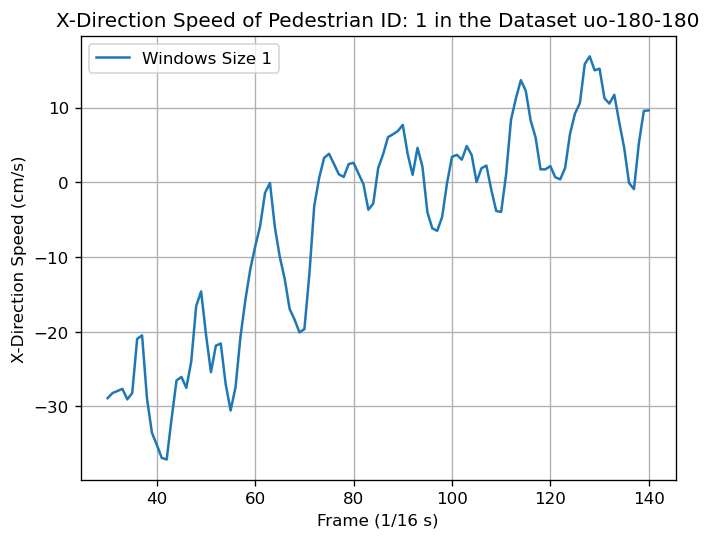
\includegraphics[width=0.32\textwidth]{images/first pedestrian speed x.png}}
\subfigure[]{
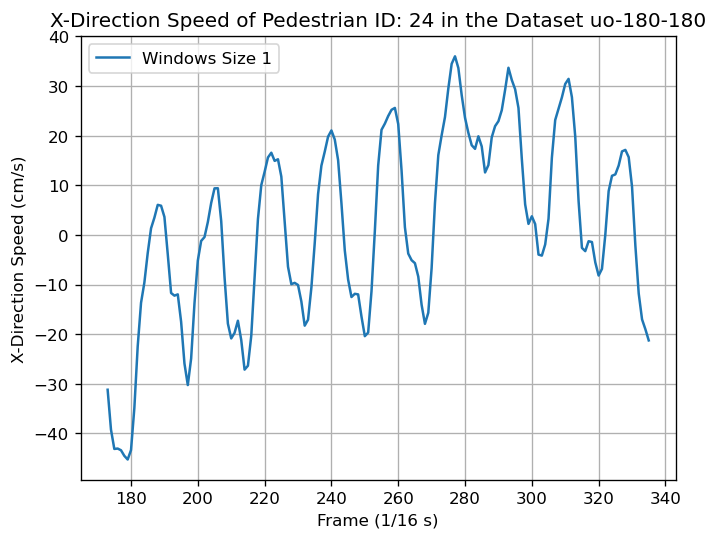
\includegraphics[width=0.32\textwidth]{images/24 pedestrian speed x.png}}
\subfigure[]{
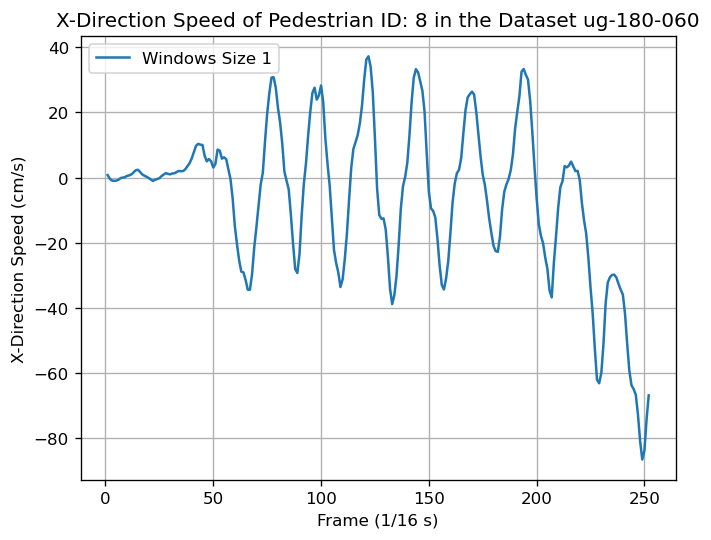
\includegraphics[width=0.32\textwidth]{images/8 pedestrian speed x.png}}
\subfigure[]{
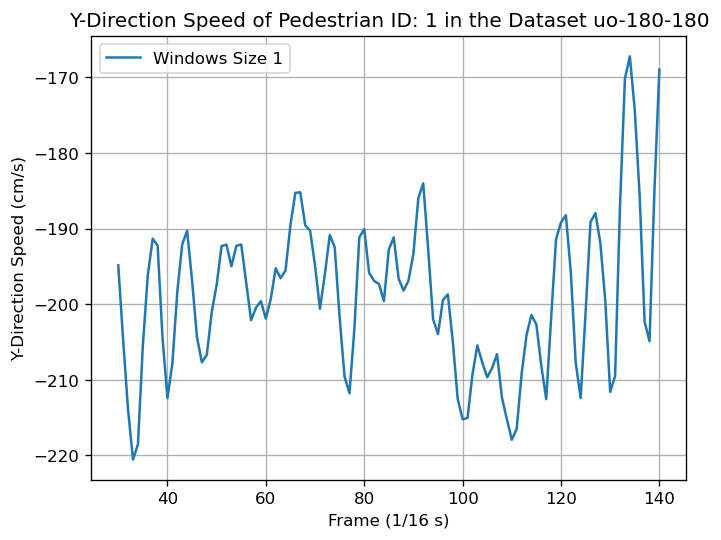
\includegraphics[width=0.32\textwidth]{images/first pedestrian speed y.png}}
\subfigure[]{
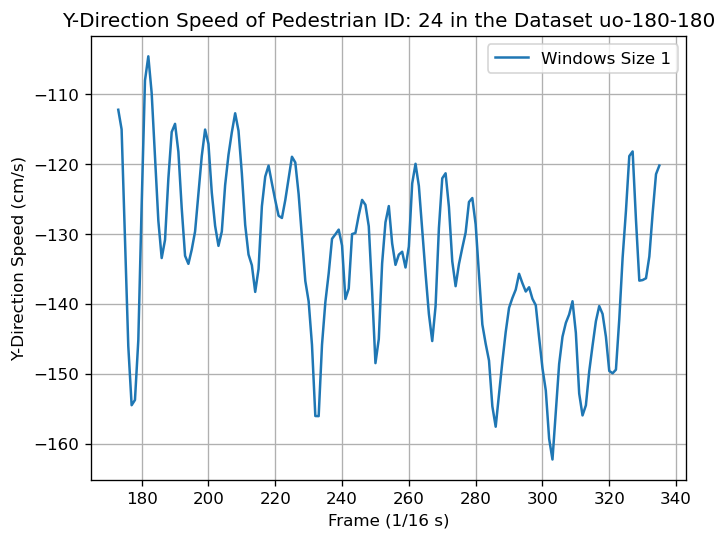
\includegraphics[width=0.32\textwidth]{images/24 pedestrian speed y.png}}
\subfigure[]{
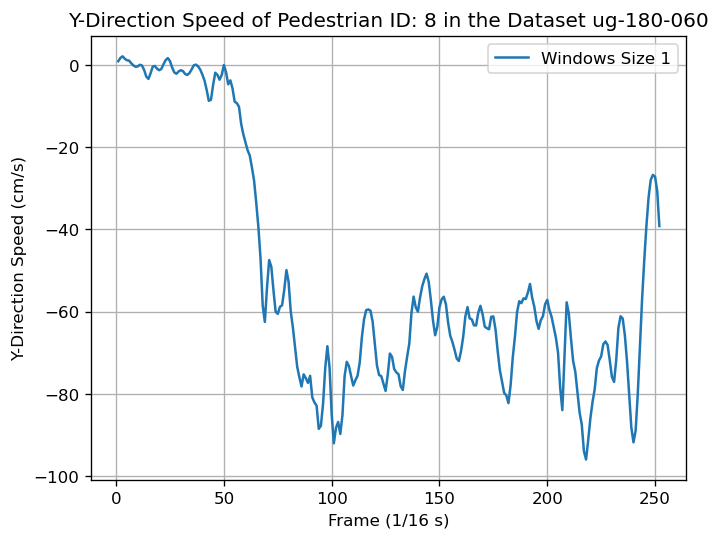
\includegraphics[width=0.32\textwidth]{images/8 pedestrian speed y.png}}
\caption{Speed of Pedestrians}
\label{pedestrain speed}
\end{figure}

By observing the figure, we can see that the pedestrian undergoes significant changes in velocity within one second. In the beginning, this change in velocity seemed very peculiar to us in some instances. For example there is nothing obstructing the first pedestrian so theoretically his velocity shouldn't be fluctuating. If the change in velocity is not influenced by external factors, then the reason for the velocity variation can only come from the individual itself. After reviewing a large number of pedestrians in the database, we found that almost every pedestrian exhibits similar velocity variations. This situation has let us to start considering the process of walking motions.

If people's walking speed variation follows a smooth curve, they should appear as if gliding on a skateboard rather than walking in a normal manner. Taking this into consideration, coupled with the fact that the data capture point are on the tester's head, we found the reason for the speed variation—when people walk, the alternating use of left and right feet causes lateral speed changes. Speed slows down when the foot is extended and accelerates when taking a step forward, resulting in longitudinal speed variations.

However, these speed changes, caused by these movement motion, are not related to avoiding pedestrians. These circumstances lead to a significant amount of noise in the data, making it challenging for our simple network to capture patterns of avoiding pedestrians. This is the reason for the high test loss.

In the Bottleneck Data dataset, we attempted to set the x-direction velocity to 0, assuming pedestrians wouldn't sway left or right, surprisingly achieving a smaller test loss. Therefore, in further data preprocessing, we intend to minimize the impact of walking motions and focus on the influence of pedestrians on the speeds of other pedestrians.

Then, we tried a larger sliding window. Figure \ref{pedestrain speed large win} compares the velocities generated using sliding windows of sizes 1, 8, and 16. The generated speed correspond to average speeds within 2/16 seconds, 16/16 seconds, and 32/16 seconds, respectively.

\begin{figure}[H]
\centering
\subfigure[]{
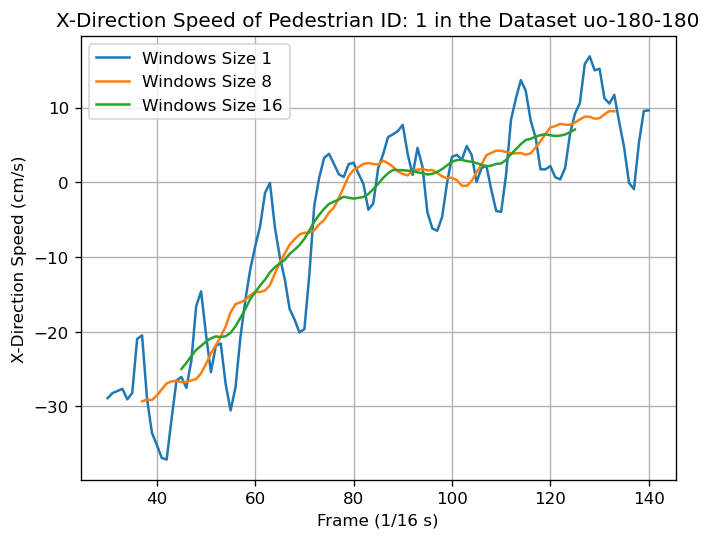
\includegraphics[width=0.32\textwidth]{images/first pedestrian speed x win.png}}
\subfigure[]{
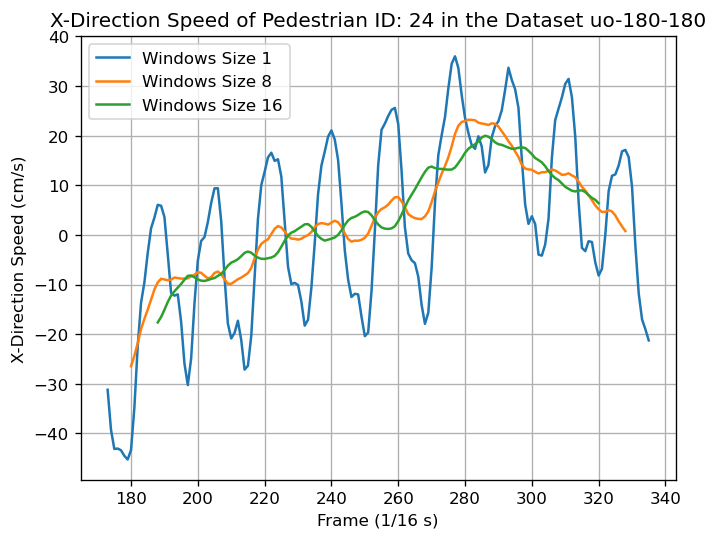
\includegraphics[width=0.32\textwidth]{images/24 pedestrian speed x win.png}}
\subfigure[]{
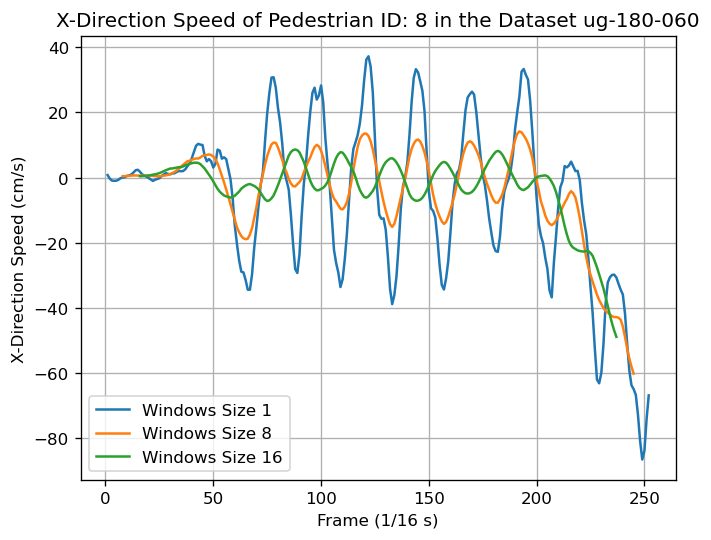
\includegraphics[width=0.32\textwidth]{images/8 pedestrian speed x win.png}}
\subfigure[]{
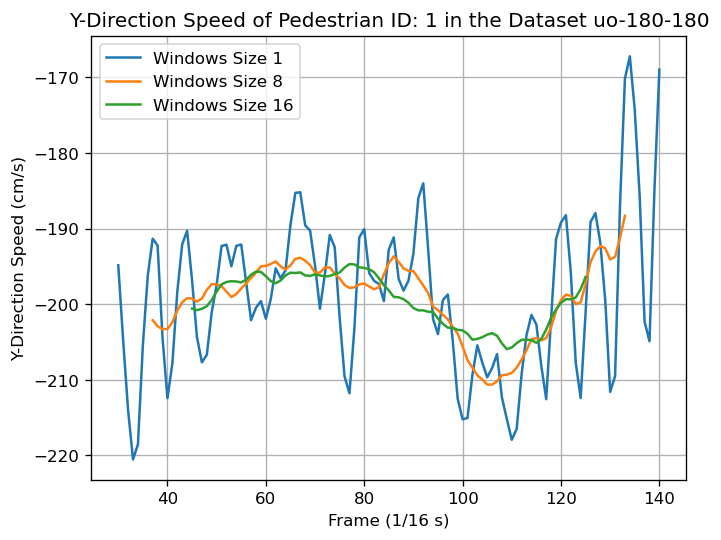
\includegraphics[width=0.32\textwidth]{images/first pedestrian speed y win.png}}
\subfigure[]{
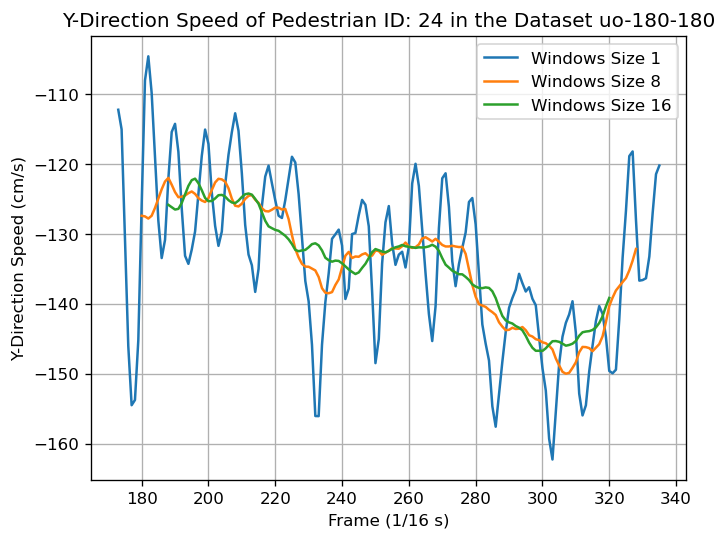
\includegraphics[width=0.32\textwidth]{images/24 pedestrian speed y win.png}}
\subfigure[]{
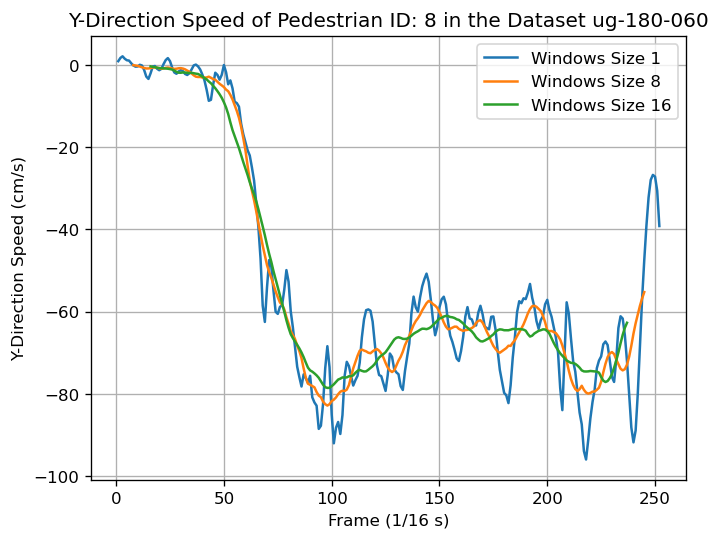
\includegraphics[width=0.32\textwidth]{images/8 pedestrian speed y win.png}}

\caption{Speed of Pedestrians}
\label{pedestrain speed large win}
\end{figure}

From the graph, it can be observed that even with a very large window size, the speed in x direction still exhibits fluctuations. Other pedestrians are not running and are unlikely to appear instantly beside the current pedestrian, so the speed variation should be smoother. This leads us to consider another method for handling the x direction of velocity. Because speed is the distance covered by pedestrians in a unit of time, we started considering whether the path of pedestrians is smooth.

Figure \ref{pedestrain path} illustrates the trajectory changes in the x and y directions for pedestrian ID 1 and ID 24 and pedestrian ID 8 in the ug-180-060, respectively. 

\begin{figure}[H]
\centering
\subfigure[]{
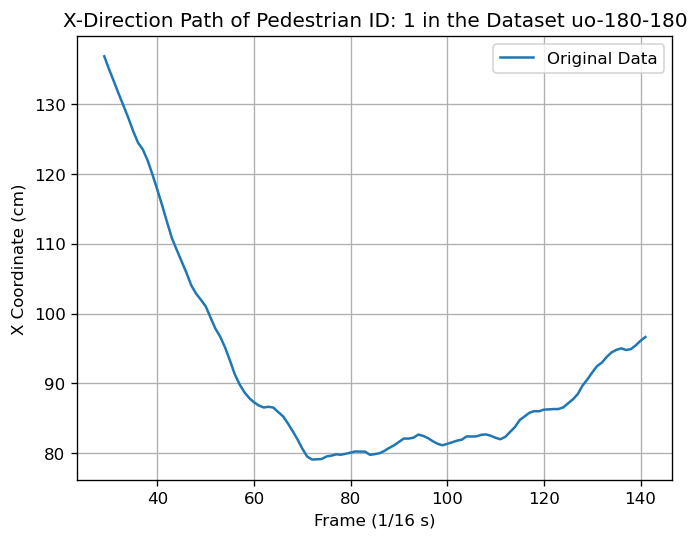
\includegraphics[width=0.3\textwidth]{images/frist pedestrian path x}}
\subfigure[]{
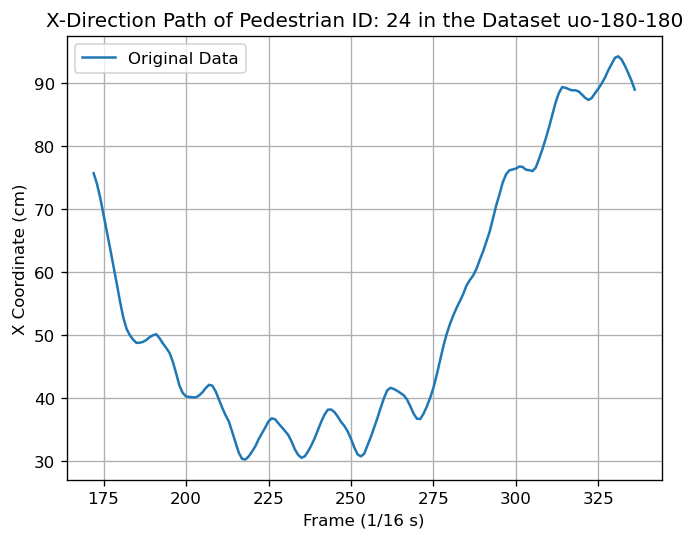
\includegraphics[width=0.3\textwidth]{images/24 pedestrian path x.png}}
\subfigure[]{
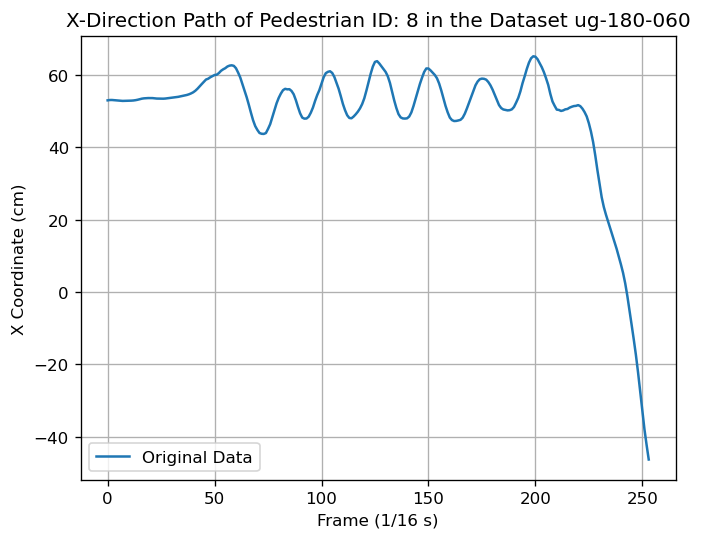
\includegraphics[width=0.3\textwidth]{images/8 pedestrian path x.png}}
\subfigure[]{
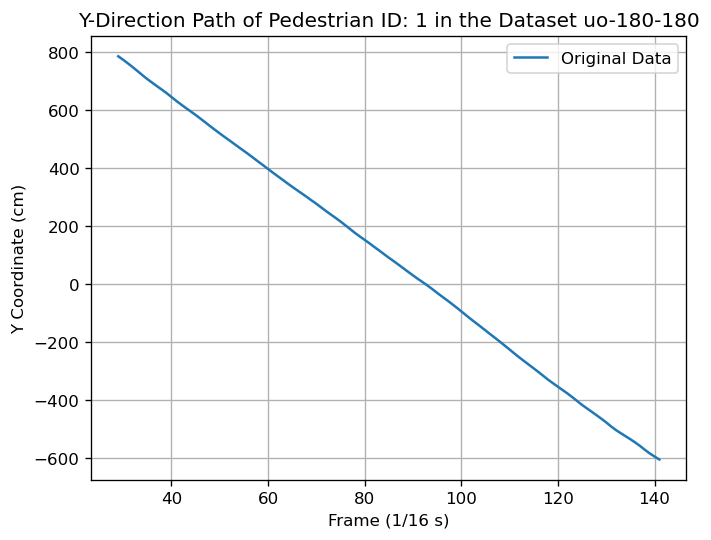
\includegraphics[width=0.3\textwidth]{images/first pedestrian path y.png}}
\subfigure[]{
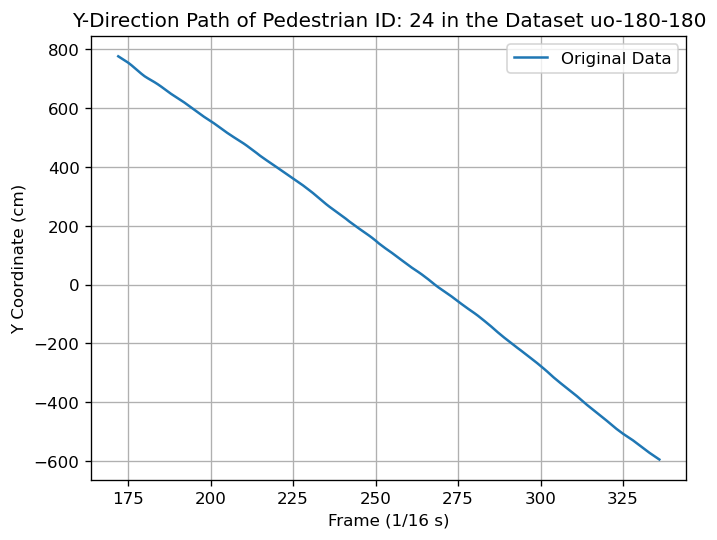
\includegraphics[width=0.3\textwidth]{images/24 pedestrian path y.png}}
\subfigure[]{
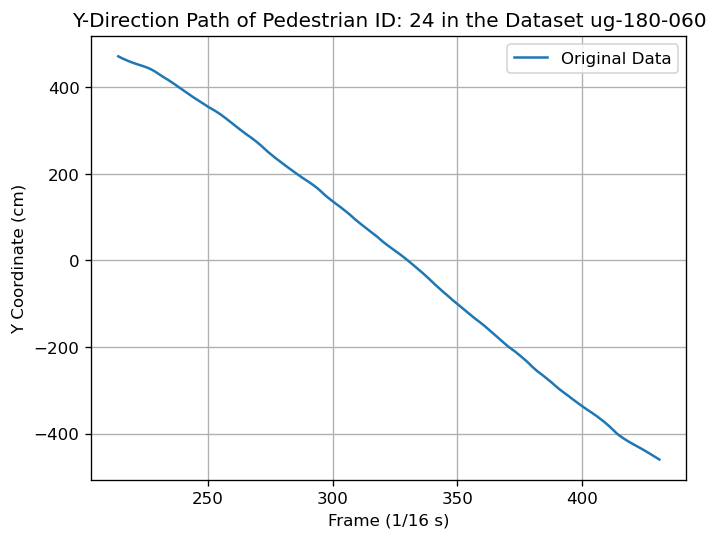
\includegraphics[width=0.3\textwidth]{images/8 pedestrian path y.png}}
\caption{Path of Pedestrians}
\label{pedestrain path}
\end{figure}

The behavior of most other pedestrians in the database is similar to the showcased pedestrians. As observed, while the trajectory is very smooth in the y-direction in both databases, there are fluctuations in the x-direction. Especially when trying to maintain the x-value, there is significant fluctuation in x. In other words, when pedestrians are walking straight forward, there is lateral swinging. To eliminate the impact of pedestrians' swinging on the data, we can fit a polynomial function to the trajectory. While the trajectory in the y-direction is smooth, no processing is needed.

Figure \ref{pedestrain path fit} shows the x-trajectory curve fitted with a polynomial function of degree 6.
\begin{figure}[H]
\centering
\subfigure[]{
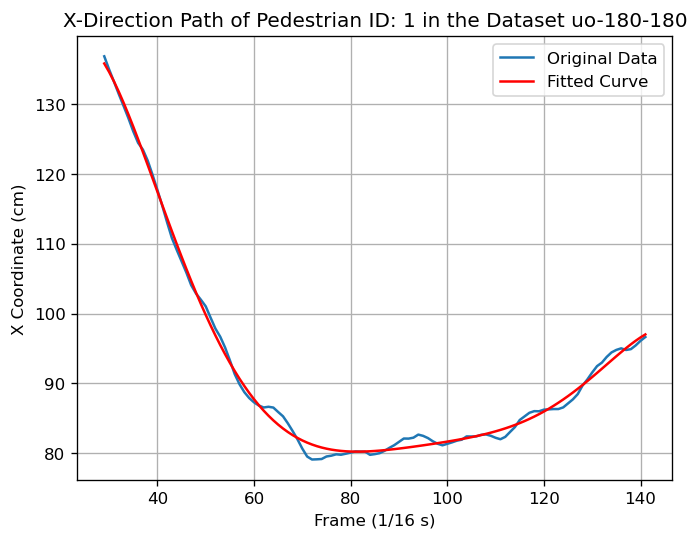
\includegraphics[width=0.3\textwidth]{images/frist pedestrian path x fit.png}}
\subfigure[]{
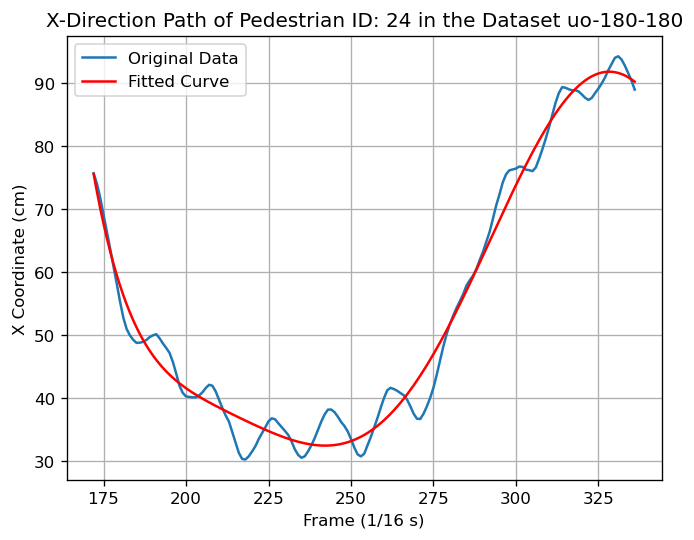
\includegraphics[width=0.3\textwidth]{images/24 pedestrian path x fit.png}}
\subfigure[]{
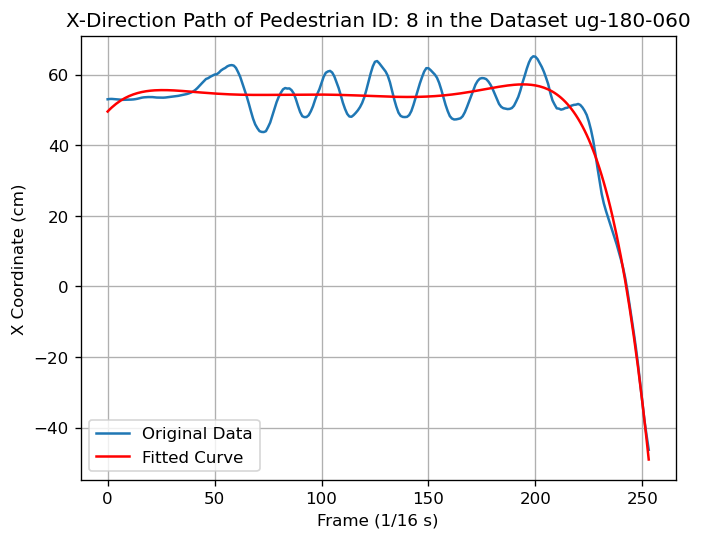
\includegraphics[width=0.3\textwidth]{images/8 pedestrian path x fit.png}\label{c}}
\caption{Fitted Path of Pedestrians in x Direction}
\label{pedestrain path fit}
\end{figure}

After this processing, the trajectory becomes significantly smoother, offering a seemingly more accurate representation of pedestrian paths. Simultaneously, it's worth noting, as observed in Figure \ref{c}, that this processing method has minimal impact on the trajectories when pedestrians make turning movements.


Using the fitted curve as the new x-direction trajectory, and then calculating the x direction speed with a sliding window of size 1, the speed curve is shown in Figure \ref{pedestrain speed fit}.

\begin{figure}[H]
\centering
\subfigure[]{
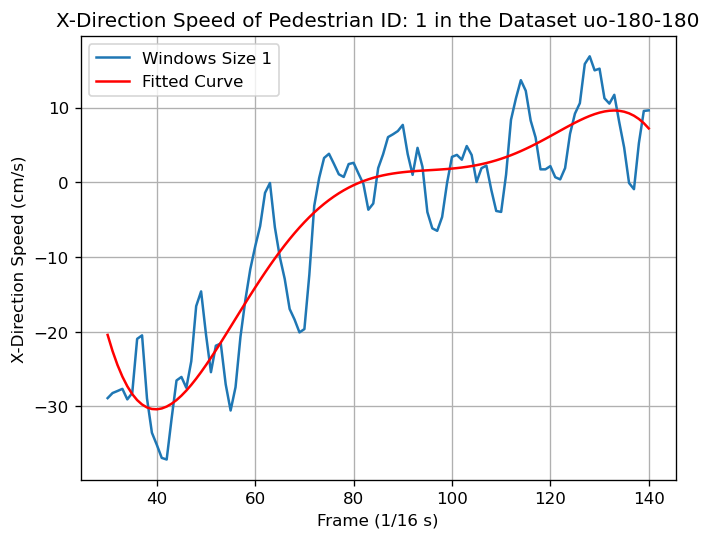
\includegraphics[width=0.3\textwidth]{images/frist pedestrian speed x fit.png}}
\subfigure[]{
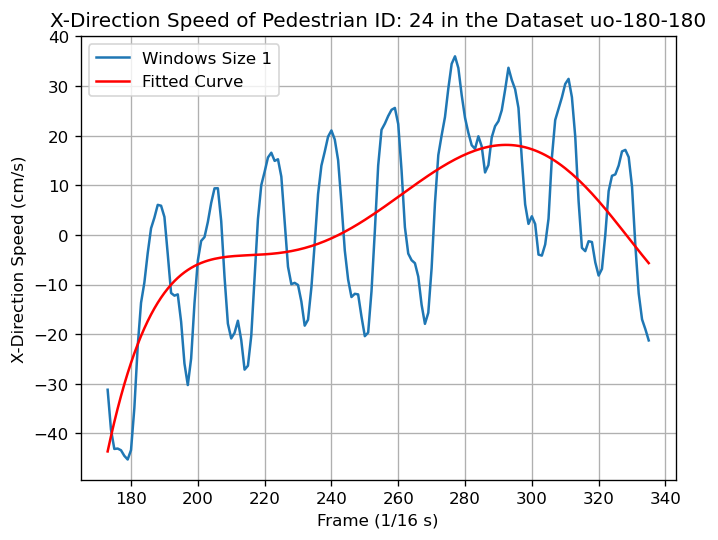
\includegraphics[width=0.3\textwidth]{images/24 pedestrian speed x fit.png}}
\subfigure[]{
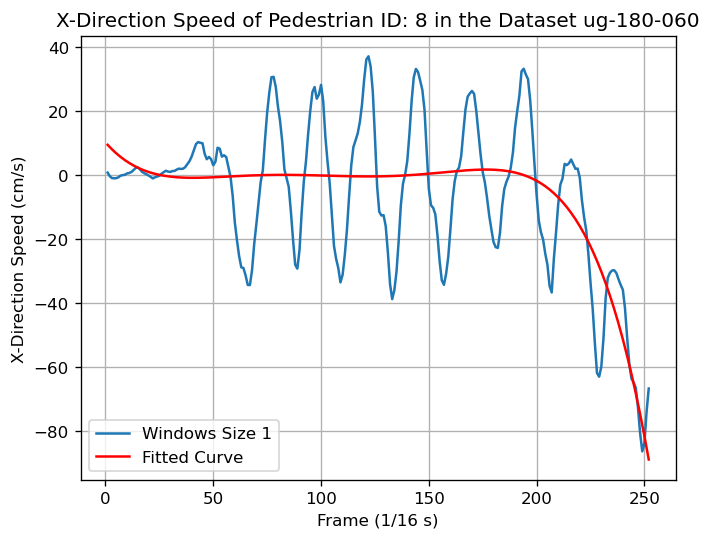
\includegraphics[width=0.3\textwidth]{images/8 pedestrian speed x fit.png}}
\caption{Fitted Speed of Pedestrians in x Direction}
\label{pedestrain speed fit}
\end{figure}

For the y-direction, since the path is very smooth and the sliding window method performs very well, there is no need to use this method. Therefore, a sliding window with a size of 8 was employed.

In this approach, We set the value of \(k\), representing the number of neighbors, to 10. when the number of people around a pedestrian is less than 10, such data is not considered because $S_k$ as well as $(x_i-x, y_i-y, v_i-v, u_i-u, 1 \leq i \leq K)$ could be inaccurately estimated. However, each individual's contribution to velocity calculation is not equal among the 10 neighbors. The influence of the closest neighbors on pedestrian velocity is expected to be more significant. Therefore, during the data preprocessing stage, we sorted pedestrians from the nearest to the farthest. This ensures that data for \(x_0, y_0, v_0, u_0\) always originates from the closest pedestrian, while data for \(x_9, y_9, v_9, u_9\) always comes from the farthest pedestrian. Features are sorted based on distance and then input to the corresponding neurons in the network. This facilitates the model in learning patterns related to the proximity of pedestrians more effectively.

Thus, we have acquired the data points utilized for training the neural network. From the Bottleneck and Corridor datasets, we obtained 240,186 and 791,023 data points, respectively.

\paragraph{Network Training}

In our initial experiments, we attempted to use the same neural network architecture as described in the paper. Let \(a\) and \(b\) denote the number of neurons in the first and second layers, respectively. Define the hidden layers as \(h = (a, b)\) (or simply \(h = (a)\) if \(b = 0\)). The evaluated hidden layers \(h\) consist of \((2)\), \((3)\), \((4, 2)\), \((5, 2)\), \((5, 3)\), \((6, 3)\), and \((10, 4)\). We chose to only train the NN4 network with an input size of 4*K+1, as it demands the maximum number of input features. This is more advantageous for uncovering differences before and after applying our data preprocessing method.


In the upcoming sections, the initial parameter X in the notation 'X/Y' indicates the dataset utilized during the training phase, with the subsequent parameter Y representing the dataset employed for the testing phase.

For B/B, C/C, and C+B/C+B, both training and testing are conducted. The data is partitioned into a 6:2:2 ratio, serving as the training set, validation set, and test set. For B/C and C/B, these scenarios are designed to assess the model's predictive capability in novel situations. The training data is split into an 8:2 ratio for the training set and validation set, with the other dataset employed as the test set. As for C+B/B and C+B/C, initially, the dataset is divided into a 7:3 ratio, with 3 reserved for testing. The remaining 7 are combined with another dataset and further divided into an 8:2 ratio, with 2 allocated for the validation set.

Before inputting the data into the network, we use the torch dataloader's shuffle function to randomize the training data sequence and set the batch size to 32. We employed Mean Squared Error (MSE) as the loss function. The optimizer utilized for training is Adam with a learning rate of 0.001.

During the training of the network, we observed that a simple network converges rapidly, stabilizing within the two epochs. This could be attributed to the abundance of data. Because we need to test six different networks across seven data scenarios, the total number of networks to be trained amounts to 56. Therefore, we have to use a relatively small number of epochs to save time. The training epoch for all networks is set to 3.

\paragraph{Result}
Due to time and computing limitations and the abundance of data, cross-validation was not implemented in this section. The network underwent training only once. The results can be observed in Figure \ref{result_2_1}.

\begin{figure}[H]
\centering
\subfigure[]{
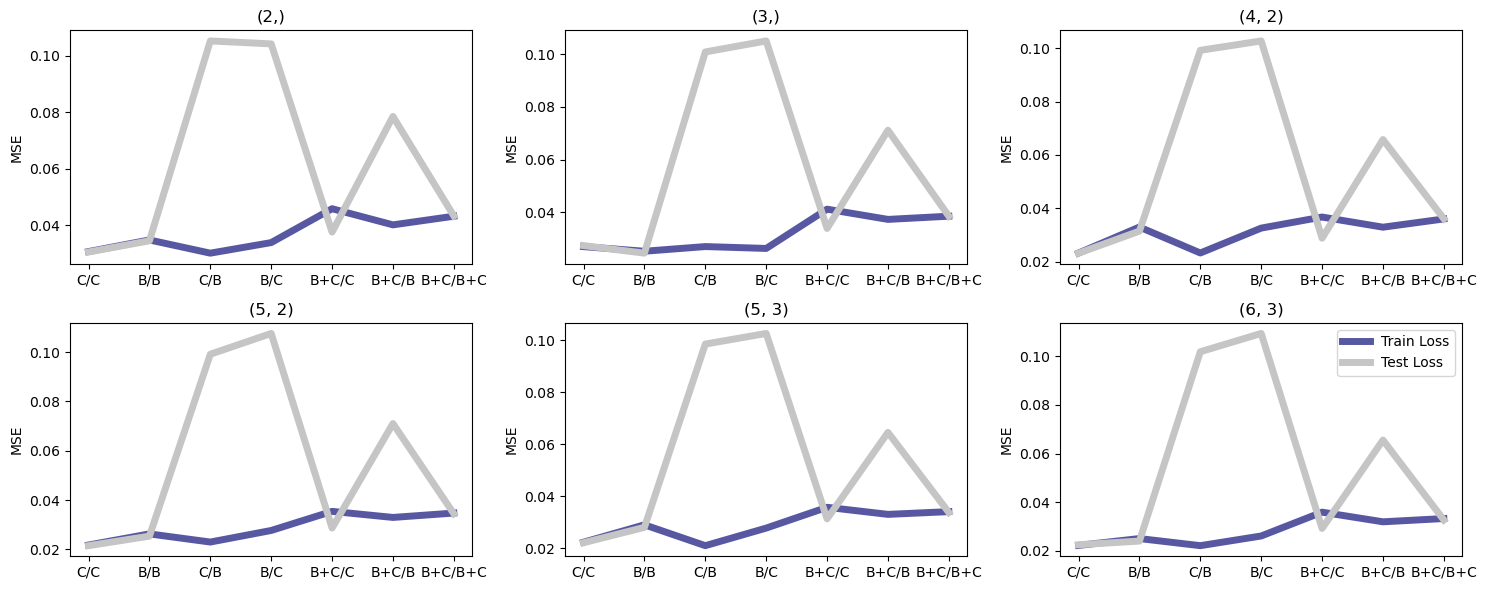
\includegraphics[width=0.95\textwidth]{images/result2.1.png }}
\subfigure[]{
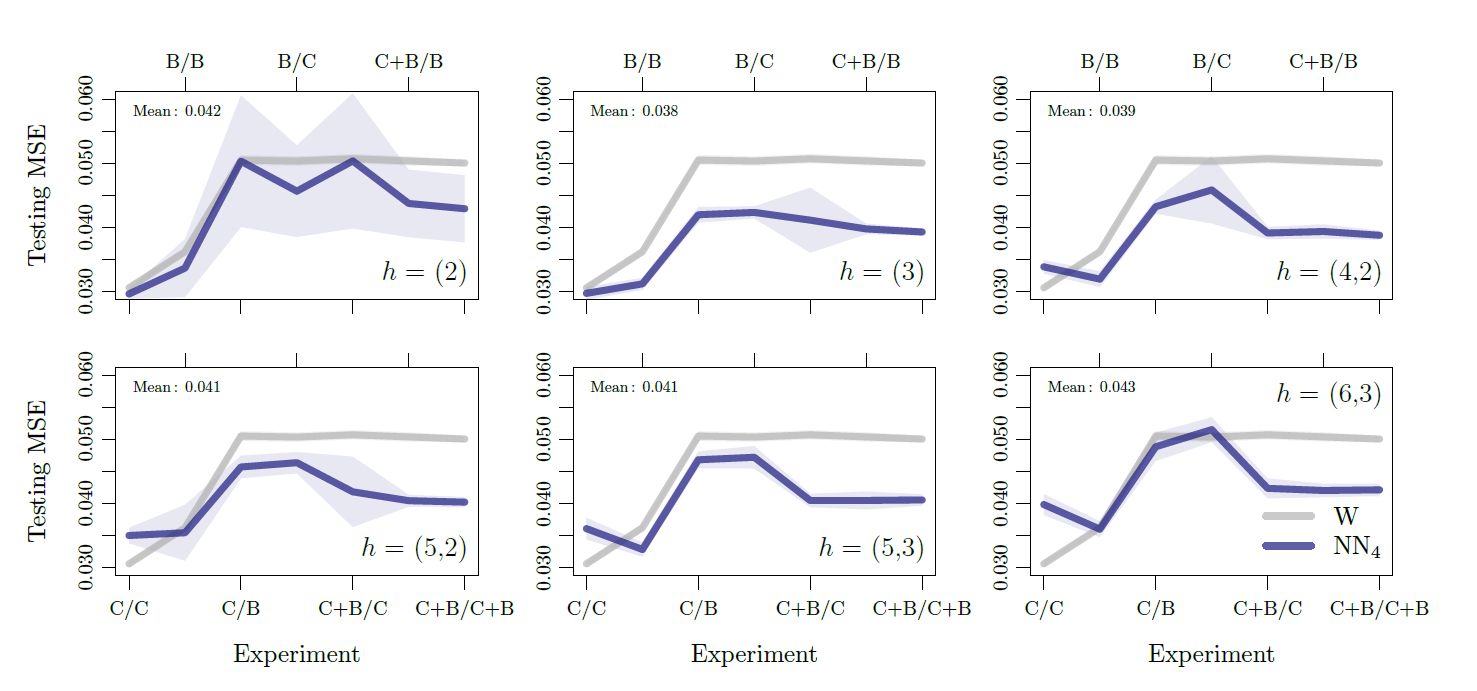
\includegraphics[width=0.95\textwidth]{images/paper result.png}}
\caption{Result}
\label{result_2_1}
\end{figure}

The upper portion of the figures is generated from our result, while the lower part is from the paper. It can be observed that in certain scenarios, our performance surpasses that of the paper, while in others, it falls short. However, we only trained for 3 epochs. If each network could be trained until the validation loss starts to rise, it is highly likely that the performance in scenarios other than C/B, B/C, and C+B/B would significantly outperform the paper. The sub-optimal performance on C/B and B/C scenarios may be attributed to the removal of noise, which we suspect leads to a slight loss of information, hindering the model's generalization to unknown datasets.

The model's performance in the C+B/B scenario is not satisfactory, and we suspect it is due to data imbalance. It might be beneficial to discard a portion of the excessive C data, achieving a balance by training the network with an equal quantity of B and C data. With this mindset, we utilized the (5,3) architecture and conducted training for 20 epochs on C+B/B with an equal number of data points for C and B. The resulting test loss was 0.063. However, this was hardly any improvement compared to the previous attempt. This did not align with our expectations. Therefore, we trained with the same architecture and epoch count without discarding any data points, yielding a test loss of 0.056. While there was some improvement, it still falls short of the results in the paper. We can roughly conclude that our data preprocessing method has had a certain impact on the generalization ability of the trained model.

During the experimentation process, we observed that the network described in the paper appears to be too simplistic, posing challenges in capturing intricate patterns. Even when attempting to overfit a simple network (3,) with a minimal number of data points, such as 500 data points, achieving a loss close to zero proves difficult. This implies limitations in the model's memorization capabilities. Consequently, we experimented with a significantly larger network (256,128,64,32) on C+B/C+B with 60 epochs, and the obtained test loss is 0.007. And on B/B with 50 epochs, the test loss is 0.006. This confirms our speculation that choosing larger models could result in more precise speed predictions.



\paragraph{Future Considerations}
In the existing dataset, the pedestrian movement is relatively uni-direcrtional. Perhaps in subsequent attempts, data augmentation techniques could be employed. For instance, rotating the coordinates around any angle axis could cause pedestrians to face different directions, significantly increasing the number of data points.

Due to the varying impact of nearby pedestrians at different distances, with the closest pedestrians having the most significant influence on the current pedestrian, it is challenging for the simple network we are using to identify this. Introducing an attention mechanism may help the model focus its attention on pedestrians in very close proximity. This, at the very least, could result in faster convergence speed for the model and potentially even lead to better results.



\paragraph{Conclusion}
Our Data preprocessing method can eliminate noise from the raw data, making it easier for the model to learn patterns. This not only leads to faster convergence of the loss function but also results in a smaller test loss. However, it may not necessarily contribute to enhancing the model's ability to generalize predictions on unknown datasets.

\end{task}